\documentclass{beamer}

\usepackage{fancyvrb}
\usepackage{color, colortbl}
\usepackage{listings}
\usepackage{url}
\usepackage{array}
\usepackage{calc}
\usepackage{ctable}
\usepackage{amsmath}
\usepackage{cite}
\usepackage{graphicx}
\usepackage{listings}
\usepackage{xspace}
\usepackage{hyperref}
\usepackage{subfigure}

\definecolor{lightgray}{rgb}{0.9,0.9,0.9}

\lstset{ %
language=C++,                % choose the language of the code
basicstyle=\tiny,       % the size of the fonts that are used for the code
%numbers=left,                   % where to put the line-numbers
numbers=none,                   % where to put the line-numbers
numberstyle=\scriptsize,      % the size of the fonts that are used for the line-numbers
stepnumber=1,                   % the step between two line-numbers. If it's 1 each line will be numbered
numbersep=15pt,                  % how far the line-numbers are from the code
backgroundcolor=\color{lightgray},  % choose the background color. You must add \usepackage{color}
%backgroundcolor=none,  % choose the background color. You must add \usepackage{color}
showspaces=false,               % show spaces adding particular underscores
showstringspaces=false,         % underline spaces within strings
showtabs=false,                 % show tabs within strings adding particular underscores
frame=single,	                % adds a frame around the code
%frame=none,	                % adds a frame around the code
tabsize=2,	                % sets default tabsize to 2 spaces
%captionpos=b,                   % sets the caption-position to bottom
captionpos=n,
%basicstyle=\small,
%basicstyle=\small\sffamily,
basicstyle=\sffamily\small,
%basicstyle=\ttfamily\small,
breaklines=true,                % sets automatic line breaking
breakatwhitespace=false,        % sets if automatic breaks should only happen at whitespace
columns=fullflexible,
title=\lstname,                 % show the filename of files included with \lstinputlisting; also try caption instead of title
escapeinside={\%*}{*)},          % if you want to add a comment within your code
morekeywords={chare,mainchare,module,mainmodule,entry,readonly,array,atomic,for,when,if,then,else,overlap,while,forall},
aboveskip=2pt,
belowskip=2pt,
lineskip=0pt,
xleftmargin=1em,
xrightmargin=1em,
%xleftmargin=10pt
abovecaptionskip=0pt,
belowcaptionskip=0pt,
}

\newcommand{\code}[1]{\colorbox{lightgray}{\texttt{#1}}}
\DefineVerbatimEnvironment{codeverb}{Verbatim}{fontsize=\small}

\hypersetup{
    colorlinks,%
    citecolor=black,%
    filecolor=black,%
    linkcolor=black,%
    urlcolor=magenta
}

\usefonttheme{professionalfonts}
\usetheme{Boadilla}
\usecolortheme{beaver}


\begin{document}

\begin{frame}[fragile]

  \frametitle{Title of the Slide}

  \begin{itemize}
    \item point 1
      \begin{itemize}
      \item point 1.a
        \begin{itemize}
        \item point 1.a.i
        \item point 1.a.ii
        \end{itemize}
      \item point 1.b
      \end{itemize}
    \item point 2
  \end{itemize}
\end{frame}

\begin{frame}[fragile]
  \frametitle{Code Segment}

  \begin{lstlisting}[basicstyle=\footnotesize]
    for (remoteCount = 0; remoteCount < 6; remoteCount++) {
        when updateGhosts[i](int i, int d, int w, int h, double b[w*h])
        atomic { updateBoundary(d, w, h, b); }
    }
  \end{lstlisting}

\end{frame}

\begin{frame}[fragile]
  \frametitle{Column Layout w/image}

  \begin{columns}
    \begin{column}{0.6\textwidth}
      \begin{itemize}
      \item Overlap can be used to get back some of the asynchrony within a chare
        \begin{itemize}
        \item But it is constrained
        \item Makes for more disciplined programming, 
          \begin{itemize}
          \item with fewer race conditions
          \end{itemize}
        \end{itemize}
      \end{itemize}
    \end{column}
    \begin{column}{0.4\textwidth}
      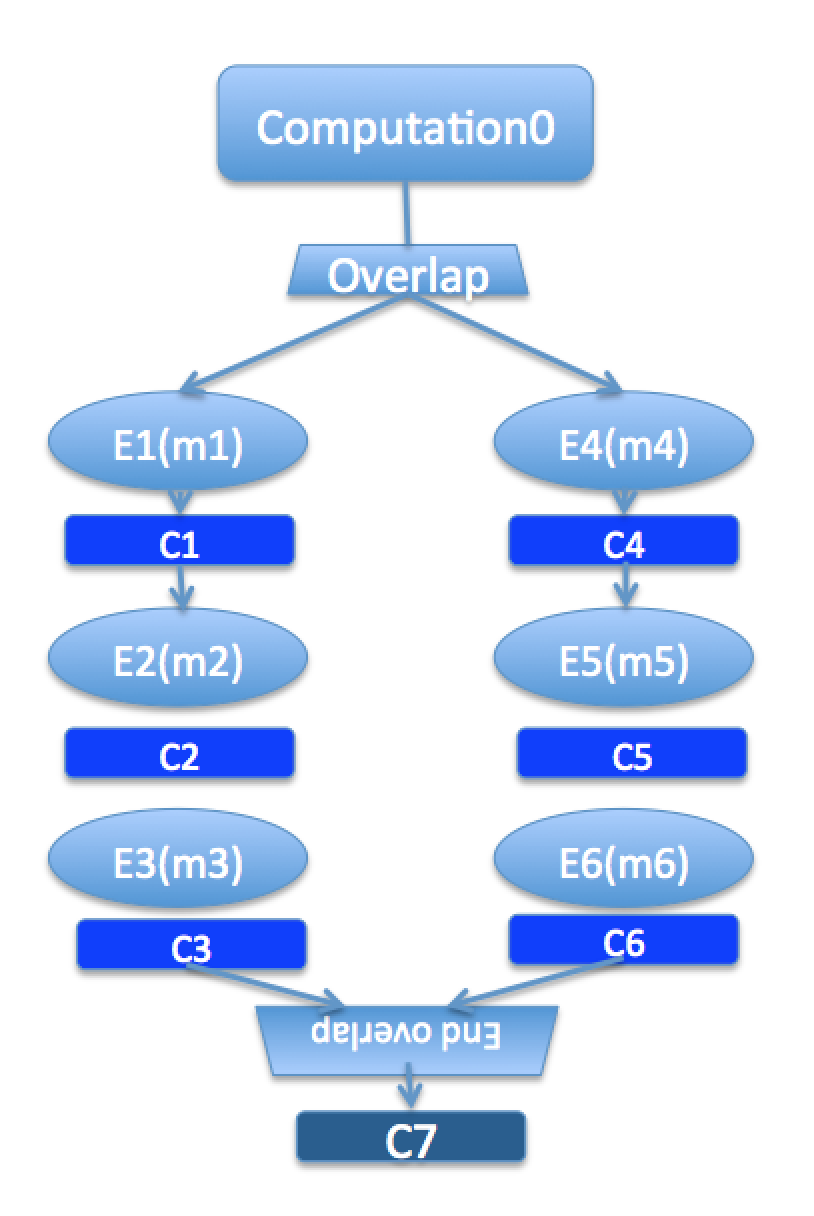
\includegraphics[width=0.8\textwidth]{classSlides/diagrams/overlapFlow.png}
    \end{column}
  \end{columns}

\end{frame}

\begin{frame}[fragile]
  \frametitle{Code Segment from File}
  \lstinputlisting[basicstyle=\tiny,linerange={22-49}]{classSlides/code/jacobi3dSYNC.ci}
\end{frame}


\end{document}